\documentclass[a4paper, 11pt, oneside]{report}

\usepackage[T1]{fontenc}    % fornisce la codifica adatta per il font della lingua italiana
\usepackage[utf8]{inputenc} % interpreta i caratteri immessi dall'editor, come i caratteri accentati italiani
\usepackage[italian]{babel} % convenzione per date, capitolo invece di chapter, regole di formattazione...

\usepackage{geometry}       % gestisce il layout del documento
% heightrounded modifica le regole di contenimento del testo per far rientrare il testo in un numero finito di righe
\geometry{a4paper, top=2cm, bottom=2cm, left=2.5cm, right=2.5cm, heightrounded}

\pagestyle{plain}           % numeri di pagina in fondo

\usepackage{hyperref}       % usato per collegamenti ipertestuali
\usepackage{graphicx}       % usato per inserire immagini
\hypersetup{hidelinks}      % usato per rimuovere i riquadri dai link

% autostyle adatta lo stile delle citazioni alla lingua del documento,
% italian=gillments racchiude tra le virgolette caporali i campi che prevedono le virgolette
\usepackage[autostyle,italian=guillemets]{csquotes}
% usato per la generazione rif bibliografici, richiede l'uso di babel e csquotes, biblatex è il motore usato.
% Le citazioni sono definite in termini di etichette numeriche come [1],[2],...
\usepackage[bibstyle=numeric, citestyle=numeric-comp]{biblatex}

\usepackage{quoting}        % usato per citazioni
\usepackage{algpseudocode}  % usato per scrivere pseudo codice
\usepackage{algorithm}
\usepackage{amsmath}

% preambolo
\title{
\includegraphics[width=0.4\textwidth]{logo}\\WeatherStyle\\Corso Fondamenti di Intellingenza Artificiale\\Prof. F.Palomba}
\author{Repository github:\\\url{https://github.com/frankzamma/NC22_WeatherStyle_classe03.git}\\\\
        \\Aurucci Raffaele\\Miglino Annalaura\\Palmieri Angelo\\Zammarrelli Francesco Giuseppe}
\date{}

\begin{document}

    % sezione dedicata al preambolo
    \begin{titlepage}
        \maketitle
    \end{titlepage}

    % produzione dell'indice automatica
    \tableofcontents

    \part{Introduzione}
        \chapter{Cos'è WeatherStyle?}

            \section{Le motivazioni}
            Il progetto Weather Style nasce dall'idea di 4 studenti pendolari dell'Università degli Studi di Salerno per
            risolvere uno dei principali problemi che si trovano ogni giorno ad affrontare.\\
            In particolare, essi ogni giorno si spostano dalla loro residenza per andare
            a seguire corsi (o svolgere esami) presso il Campus di Fisciano e devono scegliere l'abbigliamento
            che sia più adatto per fronteggiare le condizioni climatiche previste.
            Il problema esposto non riguarda solo gli studenti ma anche tutti coloro che devono spostarsi per lavoro
            verso un'altra città, quindi un applicativo che lo risolva, seppur parzialmente,
            potrebbe aiutare un significativo numero di persone.

            \section{Gli obbiettivi}
            L'obiettivo che Weather Style vuole raggiungere è quello di creare un agente intelligente che riesca a fornire
            all'utente dei suggerimenti sui capi d'abbigliamento che ritiene più adatti, questo basandosi su alcune informazioni
            metereologiche come la temperatura percepita, il clima e la stagione in cui è effettuata la previsione.

            \section{Specifiche PEAS}
            L'acronimo PEAS sta per: Performance Environment Actuators Sensors, e viene utilizzato per descrivere un ambiente.
            \begin{itemize}
                \item \textbf{P (Performance)}: è la misura di prestazione adottata per valutare l'operato di un agente.
                Nel caso di WeatherStyle, la misura di prestazione è data dal consigliare in maniera adeguata i vari capi
                d'abbigliamento.
                \item \textbf{E (Environment)}: è la descrizione degli elementi che formano l'ambiente. Nel nostro
                sistema, l'ambiente è costituito da un insieme di capi d'abbigliamento e dalle previsioni meteo.
                \item \textbf{A (Actuators)}: servono all'agente per poter compiere delle azioni. L'agente di WeatherStyle
                si serve di uno schermo per mostrare all'utente i capi d'abbigliamento che ritiene più adeguati.
                \item \textbf{S (Sensors)}: sono i sensori attraverso i quali l'agente riceve gli input dall'esterno. In
                questo caso, un sensore è sicuramente la tastiera per poter inserire dei capi d'abbigliamento.
            \end{itemize}


            \subsection{Caratteristiche dell'ambiente}
                \begin{itemize}
                    \item \textbf{Tipo di ambiente:} guardaroba con informazioni meteorologiche.
                    \item \textbf{Completamente osservabile:} l'agente attraverso i sensori conosce lo stato
                    completo dell'ambiente in ogni momento, ovvero, ha visione completa dei capi presenti nel guardaroba
                    e delle informazioni meteorologiche.
                    \item \textbf{Deterministico:} lo stato successivo dell'ambiente è completamente determinato dallo
                    stato corrente e dall'azione eseguita dall'agente, dunque, è un ambiente che non cambia nel tempo.
                    \item \textbf{Episodico:} l'esperienza dell'agente si divide in episodi atomici, in ogni episodio
                    esegue una singola azione e non si lascia influenzare da ciò che è accaduto precedentemente.
                    \item \textbf{Statico:} l'ambiente non cambia nel mentre che l'agente sta eseguendo le proprie azioni.
                    \item \textbf{Discreto:} l'ambiente fornisce un numero limitato di percezioni\footnote{input percepiti
                    in un dato istante} e azioni distinte\footnote{una sola azione per ogni episodio}.
                    \item \textbf{Singolo agente:} l'ambiente consente la presenza di un singolo agente\footnote{nei
                    capitoli successivi vedremo tre agenti che agiranno singolarmente con uno scopo comune}
                \end{itemize}

    \part{Tecniche di risoluzione}
        \chapter{La ricerca locale}
        Gli algoritmi di \textbf{ricerca locale} a differenza degli algoritmi di ricerca tradizionale non hanno come scopo
        quello di trovare una sequenza di azioni che porti dallo stato iniziale allo stato obbiettivo, bensì lo stato
        obbiettivo rappresenta esso stesso la soluzione al problema, indipendentemente da come ci si è arrivati.
        \par \noindent Questo rende gli algoritmi di ricerca locale particolarmente adatti a problemi di configurazione
        e/o di ottimizzazione. Sono anche detti algoritmi di ``miglioramento iterativo'', poiché partono da un'ipotetica
        soluzione con lo scopo di migliorarla, secondo quella che viene chiamata \textbf{funzione obbiettivo}, una misura
        che serve all'algoritmo per comprendere se e quanto sta migliorando nelle iterazioni, condizione fondamentale per
        la corretta terminazione dell'algoritmo.
        \par \noindent In ultimo accenniamo al fatto che le soluzioni ottenute non sempre sono soluzioni ottimali, ma il
        più delle volte soluzioni sub-ottimali, ciò è dovuto dalla mancata esplorazione dell'intero spazio degli stati;
        compito del progettista è cercare di migliorare la capacità di esplorazione dell'algoritmo.

            \section{Gli algoritmi genetici}
            Sebbene possa sembrare un argomento che si sia affacciato da poco sull'umanità, la storia degli algoritmi genetici
            ha inizio con il celeberrimo biologo inglese, Charles Darwin.
            \par \noindent Darwin pubblicò nel 1859 \textit{"L'origine della specie"}, libro che riscosse un enorme
            successo e nel quale si introduceva per la prima volta il concetto di \textbf{teoria dell'evoluzione} tramite
            un processo di \textbf{selezione naturale}.
            \par \noindent Negli anni '50 del XX secolo cominciarono a diffondersi gli algoritmi evolutivi,
            i quali usano tutti i concetti formulati dalla teoria di Darwin, ovvero:
            \textit{genotipo}, \textit{fenotipo}, \textit{individuo}, \textit{popolazione}, \textit{evoluzione} e via dicendo.
            \par \noindent
            \\ \noindent Nel vasto insieme degli algoritmi evolutivi troviamo anche gli \textbf{algoritmi genetici} che vennero
            presentati nel 1975 da John Holland, all'epoca detti \textit{genetic plans}.
            \par \noindent La definizione di algoritmi genetici è dunque la seguente:
            procedura di alto livello (meta-euristica) ispirata alla genetica per \textbf{definire}
            un algoritmo di ricerca.
            \par \noindent
            \\ \noindent Partendo da questa definizione si può dire che un algoritmo genetico evolve una \textbf{popolazione}
            di \textbf{individui} (le cosiddette soluzioni candidate) producendo un iterazione dopo l'altra delle
            soluzioni che migliorino sempre rispetto ad una \textbf{funzione obbiettivo}, fino a che non si è raggiunta
            la soluzione \textbf{ottimale} o si sia verificata una \textbf{condizione di terminazione}.
            Per poter creare nuove \textbf{generazioni} di individui bisogna applicare degli \textbf{operatori genetici},
            più nello specifico la \textbf{selezione}, il \textbf{crossover} e la \textbf{mutazione}.
            \par \noindent \newpage

            \section{Formulazione del problema}
            Formulazione del GA (codifica individui\label{codifica:ga} - spostare se necessario, vincoli\label{vincoli:ga}
            operatori genetici)
            \par \noindent Funzione di fitness (euristiche generali per il calcolo del punteggio)
            \par \noindent [potrebbe essere utile fare delle sottosezioni]

            \section{Vantaggi e svantaggi}
            La soluzione illustrata in questo capitolo presenta dei vantaggi e degli svantaggi, molti dei quali legati
            alla natura degli algoritmi genetici.
            Uno dei principali problemi affrontati è stato sulla generazione della popolazione iniziale.
            In genere, la prima popolazione viene generata in maniera totalmente casuale quindi non è detto che
            tali individui rispettino il vincolo imposto (i tre elementi devono essere diversi).\\
            Il problema è stato risolto andando ad impostare una generazione pseudo casuale della prima generazione che permette
            di avere anche nella prima generazione degli elementi ammissibili e, di conseguenza,
            la ricerca viene guidata verso soluzioni ammissibili e migliori riducendo il carico computazionale.\\

            Un'osservazione importante da fare riguarda l'efficienza.
            Con un guardaroba di grandi dimensioni, gli algoritmi genetici,
            ci permettono sicuramente di effettuare un numero inferiore di computazione rispetto ad una ricerca esaustiva
            restituendo quasi sempre buon risultato.
            Tuttavia, con il setup da noi effettuato, cioè \emph{size della popolazione = 10} e
            \emph{max = 100}, i GA diventano più efficienti della ricerca esaustiva con un numero di capi
            maggiore strettamente di 10.
            Infatti, facendo un po' di calcoli il numero di stati possibili con 10 capi è pari al numero di disposizioni
            con ripetizione di 10 elementi raggruppati in classi di 3:
            \begin{equation*}
                D_{10,3}^{'}=10^{3}=1000
            \end{equation*}
            che è esattamente uguale al numero massimo di valutazione della funzione di fitness che il GA compie durante la sua esecuzione:
            \begin{equation*}
                populationSize * maxEvaluation = 10 * 100 = 1000
            \end{equation*}
            Dunque, ha senso utilizzare l'approccio basato su algoritmi genetici quando il numero dei capi è maggiore di 10.

            \par \noindent [potrebbe essere utile fare delle sottosezioni]

            \section{Implementazione}
            Per l'implementazione della soluzione basata su algoritmo genetico è stato utilizzato il framework
            \textbf{Jenetics} \cite{1}.
                \subsection{Codifica degli individui}
                \par \noindent Per prima cosa è stato necessario definire come è fatto un individuo, secondo la logica
                del framework quando si parla di individuo, esso è chiamato \textbf{Genotype}, a sua volta composto
                da cromosomi, detti \textbf{Chromosome}, i cromosomi a loro volta sono costituiti da geni, detti
                \textbf{Gene}.
                \medskip
                \par \noindent Rispetto a ciò che è stato detto nella sezione \ref{codifica:ga} possiamo definire
                i genotipi mediante tre cromosomi, costituti da geni che a loro volta hanno al proprio interno valori
                interi che variano da \textbf{0} a \textbf{sizeCapi $-$ 1}.
                \medskip
                \begin{algorithmic}[1]
                    \State $firstChromosome \gets Gene(0,sizeCapi-1)$
                    \State $secondChromosome \gets Gene(0,sizeCapi-1)$
                    \State $thirdChromosome \gets Gene(0,sizeCapi-1)$
                    \State $genotype \gets [firstChromosome, secondChromosome, thirdChromosome]$
                \end{algorithmic}

                \subsection{Vincoli}
                \par \noindent Per quel che riguarda la definizione dei vincoli già discussi nella sezione \ref{vincoli:ga}
                il framework mette a disposizione l'interfaccia \textbf{Constraint} attraverso la quale si vanno a ridefinire
                due metodi:
                \begin{itemize}
                    \item \textbf{test():} metodo che verifica se un genotipo ottenuto in una qualsiasi iterazione è un
                    buon individuo o meno.
                    Nello specifico diremo che il test ha avuto esisto positivo se i valori interi di cui è composto il
                    genotipo sono tre valori diversi, altrimenti diremo che ha avuto esito negativo.
                    \item \textbf{repair():} metodo che viene chiamato quando un genotipo non ha superato il test e si
                    cerca quindi di ripararlo.
                    Nello specifico andremo a costruire un nuovo genotipo che rispetta il vincolo e lo assoceremo a un
                    \textbf{Phenotype}, ovvero un individuo che è stato valutato; esso viene passato in input al metodo
                    ed è costituito dal valore di fitness ottenuto e da un numero \emph{i}, ovvero la i-esima generazione
                    a cui appartiene.
                \end{itemize}

                \subsection{Funzione di fitness}
                \par \noindent Venendo alla funzione di fitness, come già descritto nella sezione \ref{fitness:ga} il
                nostro obbiettivo è quello di massimizzare il punteggio ottenuto dalla combinazione dei geni per ogni
                fenotipo.
                \par \noindent In termini semplici, per ogni individuo andremo a valutare i tre valori interi, i quali
                corrisponderanno alle posizioni dei capi d'abbigliamento in una lista, calcoleremo il punteggio per ognuno,
                faremo una media e restituiremo il risultato.

                \subsection{Operatori genetici}
                Per la risoluzione del problema sono stati scelti i seguenti operatori genetici:
                \begin{itemize}
                    \item \textbf{RouletteWheelSelector:} operatore di selezione, gli individui ricevono una probabilità
                    di selezione calcolata includendo il corrispettivo valore di fitness. L'algoritmo andrà a selezionare
                    $n$ individui, saranno consentite ripetizioni degli stessi individui.
                    \item \textbf{MultiPointCrossover:} operatore di crossover, selezionerà due punti casuali in ogni
                    individuo, scambierà il patrimonio genetico di quest'ultimi a coppie di due rispetto ai punti di
                    crossover e genererà per ogni coppia di genitori due nuovi individui figli che costituiranno la
                    successiva generazione. È stata inoltre inserita una probabilità di crossover pari a $0.25$.
                    \item \textbf{GaussianMutator:} operatore di mutazione, muterà casualmente un gene dall'individuo
                    risultante dell'applicazione del crossover, il valore del nuovo gene sarà calcolato prendendo un
                    valore definito nella distribuzione gaussiana a partire dal gene corrente.
                \end{itemize}

                \subsection{Setup dell'algoritmo}
                Dopo aver quindi dato una codifica agli individui, definiti i vincoli, la funzione di fitness e aver
                scelto gli operatori genetici è giunta l'ora di fare il setup dell'algoritmo.
                \par \noindent Nel seguente pseudo codice riassumiamo i passi fondamentali.
                \medskip
                \begin{algorithm}
                \caption{Setup genetic algorithm}
                    \label{setup:ga}
                    \begin{algorithmic}[1]
                        \State $populationSize \gets 10$
                        \State $maxEvaluation \gets 100$
                        \State
                        \State $constraint \gets ConstraintImplement()$
                        \State $selector \gets RouletteWheelSelector()$
                        \State $crossover \gets MultiPointCrossover(0.25)$
                        \State $mutator \gets GaussianMutator()$
                        \State
                        \State $geneticAlgorithm \gets setup(populationSize, maxEvaluation, genotype, fitness,$
                        \State $\hspace*{12.3em} constraint, selector, crossover, mutator)$
                    \end{algorithmic}
                \end{algorithm}

        \chapter{Il machine learning}
        Brevissima spiegazione di cos'è il machine learning

            \section{CRISP-DM}
            Per progettare una soluzione basata sul \textbf{machine learning} bisogna avere un approccio data \& software
            engineering.
            Questo è necessario perché la stragrande maggioranza dei sistemi software che non sono adeguatamente ingegnerizzati
            falliscono e rischiano di arrecare danni a cose, persone e ambiente circostante.
            \par \noindent Per avere un corretto approccio ingegneristico è possibile scegliere uno dei vari cicli di vita
            di progetti basati su intelligenza artificiale e data science, uno dei più conosciuti è il CRISP-DM ed è anche
            il modello che abbiamo adottato noi per progettare la nostra soluzione.
            \par \noindent
            \\ \noindent Il CRISP-DM (Cross-Industry Standard Process for Data Mining) è formato da diverse fasi che possono
            essere eseguite un numero illimitato di volte il che lo rende un modello \textit{non} sequenziale.
            Nelle sezioni che seguono andremo ad analizzare le fasi del CRISP-DM, mostrando cosa è stato fatto in ognuna di esse
            al fine di poter raggiungere il nostro obiettivo tramite una soluzione basata sul machine learning.
            \par \noindent
            \begin{center}
                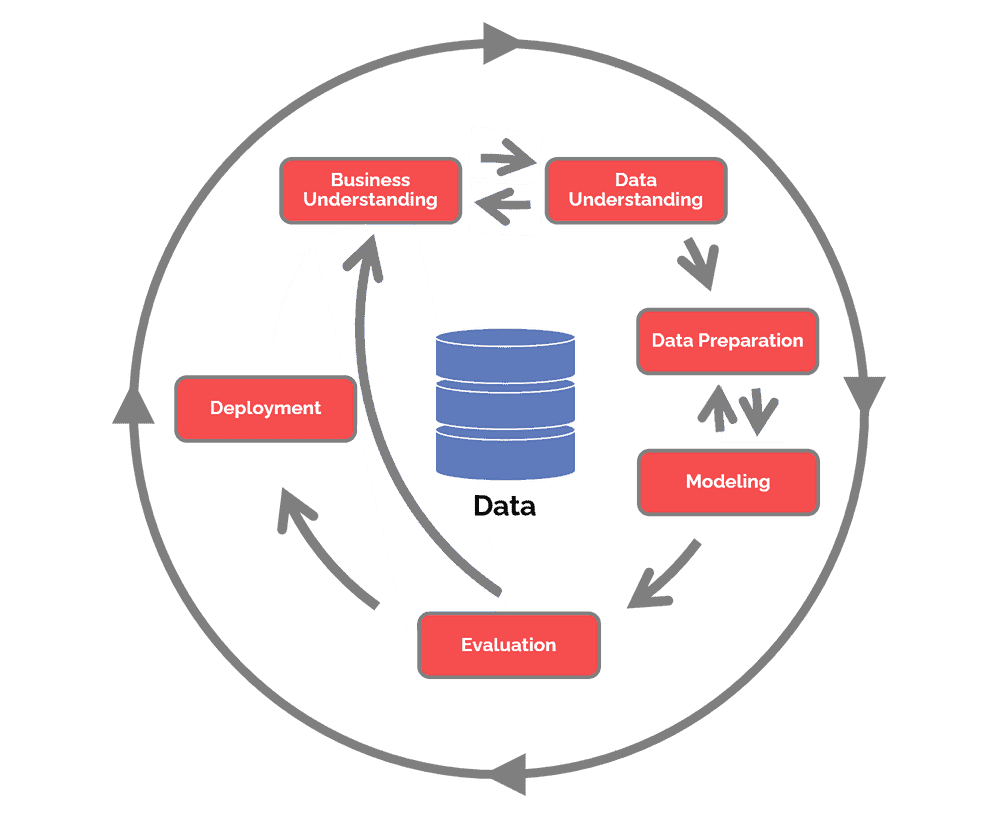
\includegraphics[scale=0.3]{CRISP-DM}
            \end{center}

            \section{Business Understanding}
            La prima fase del CRISP-DM è quella di \textbf{Business Understanding}.
            Qui si raccolgono i requisiti e si definiscono gli obiettivi di business che si intende raggiungere, oltre a
            determinare la disponibilità delle risorse, stimare i rischi, indicare le tecnologie e gli strumenti utilizzati
            per raggiungere gli obbiettivi di business.
            \par \noindent
            \begin{itemize}
                \item \textbf{Obiettivi di business}: Il machine learner che stiamo progettando avrà come obiettivo quello di
                saper stimare adeguatamente, attraverso un punteggio numerico, quali capi d'abbigliamento sono più adatti basandosi
                sulle caratteristiche dei capi e sulle informazioni metereologiche quali temperatura percepita, clima e
                stagione della previsione.
                \item \textbf{Disponibilità delle risorse}: Per raggiungere il nostro obbiettivo principale ci serviranno
                delle risorse ovvero un dataset per ogni capo d'abbigliamento (maglia, pantalone e scarpa),  
                che contiene informazioni riguardo il capo d'abbigliamento specifico e delle informazioni meteo correlate.
                \par \noindent Purtroppo dopo un'approfondita ricerca non siamo riusciti a trovare nessun dataset che facesse
                al caso nostro, anche sfruttando siti importanti nell'ambito del machine learning come \url{https://www.kaggle.com},
                quindi per rimediare a questo abbiamo costruito i dataset che ci servivano acquisendo, analizzando e modellando
                i dati da altri dataset.
                \item \textbf{Stima dei rischi}: Il non avere già in partenza dei dataset su cui poter lavorare comporta
                di certo un rischio non di poco conto dato che bisogna costruirseli da se e dunque i dati non sono adeguatamente testati.
                \item \textbf{Tecnologie e strumenti}: Per acquisire, analizzare e modellare i dati abbiamo scelto di utilizzare
                il linguaggio Python poiché mette a disposizione diverse librerie molto utili per i nostri scopi.
                L'addestramento e l'implementazione dei modelli invece è fatta in linguaggio Java, questo per comodità dato che
                l'intero applicativo di Weather Style è scritto usando tale linguaggio di programmazione.
            \end{itemize}

            \section{Data Understanding}
            Potrebbe essere utile inserire i link dei dataset trovati online e per ognuno costruire dei piccoli grafici
            (es: dataset maglie aveva dress, top e bottom e si mostra\ldots)
                \subsection{Dataset maglie e pantaloni}
                Questa fase può essere accorpata, magari si fa metà e metà
                \subsection{Dataset scarpe}
                Stesso discorso di cui sopra

            \newpage
            \section{Data Preparation}
            Qui parliamo del feature selection (feature che abbiamo selezionato), della fusione col dataset meteo e come
            è stata calcolata la variabile dipendente, eventuali imputazioni fatte\ldots
                \subsection{Dataset maglie e pantaloni}
                Per costruire i dataset contenenti le informazioni delle \textbf{maglie} e dei \textbf{pantaloni} ci siamo serviti delle
                informazioni ricavate nella fase di Data Understanding \textit{(sottosezione 3.3.1)}.
                \par \noindent Il procedimento di \textit{Data Preparation} si articola nei seguenti quattro passaggi:
                \begin{itemize}
                    \item \textbf{Data cleaning}: la cosidetta \textit{"pulizia dei dati"} si occupa di
                    rimediare a problemi che sorgono quando ci sono righe del dataset che hanno dei dati \textbf{mancanti}, ma più
                    in generale ha come obbiettivo quello di fornire un dataset dotato di una \textbf{qualità} ritenuta adeguata
                    per poter procedere con i successivi passaggi.
                    \par \noindent Nel nostro specifico caso abbiamo individuato alcuni dati mancanti in corrispondenza della
                    colonna della \textit{lunghezza della manica} (dataset maglie) e della \textit{lunghezza del pantalone}.
                    \par \noindent Si è scelto, in entrambi i casi sia per le maglie che per i pantaloni, di non andare a rimuovere
                    le colonne dai due dataset poiché le consideriamo due caratteristiche molto utili per il nostro machine learner
                    nel momento in cui dovrà effettuare delle previsioni.
                    Si è deciso, sempre in ambedue i dataset, di non andare a rimuovere le righe che avevano celle mancanti
                    perché ci si è resi conto che il numero di istanze diminuiva notevolmente.
                    \par \noindent Ci siamo dunque affidati al \textbf{data imputation}, insieme di tecniche che
                    possono stimare il valore dei dati mancanti sulla base dei dati a nostra disposizione.
                    Nello specifico abbiamo adottato la tecnica di imputazione \textit{"most frequent imputation"} che permette
                    di sostituire i dati mancanti col valore più frequente contenuto in una colonna.
                    \par \noindent Fatto ciò non si avranno più dati mancanti, successivamente abbiamo riscontrato una grande
                    diversificazione di valori nella colonna relativa al materiale, sia nelle maglie che nei pantaloni.
                    Si è dunque deciso di ricondurre questi valori ad un elenco di materiali più ristretto in modo tale da ridurre
                    la complessità in fase di addestramento e previsione.
                    Ciò è stato possibile poiché abbiamo scelto con cura il nostro elenco di materiali in modo tale che fossero;
                    quelli più comuni sul mercato, facilmente riconoscibili dagli utenti che utilizzeranno l'applicativo e
                    facilmente riconducibili all'elenco di materiali di partenza.
                    \par \noindent Inoltre si è trasformato la colonna dei colori in modo che indicasse se la maglia o il pantalone
                    fosse chiaro, scuro o colorato.
                    Questo perché il nostro obbiettivo \textbf{non} è quello di fornire un punteggio ad un determinato capo andando ad
                    analizzare le varie combinazioni di colori che si possono ottenere.
                    \par \noindent Infine si è tradotto, per una scelta convenzionale, dall'inglese all'italiano ogni valore.
                    \item \textbf{Feature scaling}: Il \textit{feature scaling} è un insieme di tecniche che permettono di
                    normalizzare o scalare l'insieme di valori di una caratteristica.
                    \par \noindent Nel caso della preparazione dei nostri dataset di maglie e pantaloni non è stata effettuata
                    il  \textit{feature scaling} poiché tutte le feature sono di tipo categorico e non numerico.
                    \item \textbf{Feature selection}:
                    \item \textbf{Data balancing}:
                \end{itemize}
                \subsection{Dataset scarpe}
                Come è stato costruito, strategia
                \subsection{Dataset meteo}
                Come è stato costruito, strategia
                \subsection{La fusione dei dataset}
                Qui si parla di come è stata calcolata la variabile dipendente, facendo riferimento alla sezione dedicata
                alla formulazione del problema per il GA in particolare alla fitness

            \section{Modelling}
            Qui parliamo della tecnica di machine learning utilizzata, ovvero la regressione e dell'algoritmo utilizzato
                \subsection{La regressione}
                Brevissima spiegazione di che cos'è la regressione
                \subsection{L'albero di regressione}
                Spiegazione teorica di un albero di regressione
                \subsection{Ten folds cross-validation}
                Spiegazione teorica del 10 folds cross validation utilizzato
                \subsection{Valutazione delle metriche}
                Qui è possibile parlare delle metriche a cui ci siamo affidati, dei risultati ottenuti per ogni modello
                e inserire i grafici che mostrano la stima dell'errore rispetto alle predizioni fatte

            \section{Evaluation}
            Qui parliamo della sperimentazione empirica e dei risultati ottenuti
            Il risultato ottenuto non è da sottovalutare sicuramente per la non disponibilità dei dati.
            In particolare valutiamo

            \section{Deployment}
            Qui si parla leggermente dell'implementazione e delle scelte ingegneristiche per rendere il modello usabile
            quindi eventuali classi interfacce, ecc\ldots


    \part{Conclusioni e osservazioni}
        \chapter{Cosa scegliamo?}
            \section{Un confronto tra GA e ML}
                Quando conviene uno e quando conviene l'altro
            \section{Possiamo fare di meglio}
                Introduzione alle due osservazioni
                \subsection{Usare il ML per il calcolo della funzione di fitness}
                Spiegare cosa si può fare
                \subsection{Usare un GA per costruire l'albero di regressione}
                Spiegare cosa si può fare


    % sezione dedicata ai riferimenti bibliografici
    \begin{thebibliography}{9} % meno di 10, 99 meno di 100 e così via...
        \bibitem{1}
        Jenetics, Java Genetic Alghorithm Library,
        \url{https://jenetics.io/}.

        \bibitem{2}
        Weka, Waikato Environment for Knowledge Analysis,
        \url{https://www.cs.waikato.ac.nz/ml/weka/}.
    \end{thebibliography}

\end{document}